\chapter{Características de SI}

\section{Aspectos Tecnológicos, Organizacionais e de Pessoas}

Para uma análise completa das características do Sistema de Informação, faz-se necessário o entendimento de suas três dimensões essenciais: organização, pessoas e tecnologia. O projeto desenvolvido é uma relevante contribuição às tecnologias de IoT e promove uma alternativa de baixo custo, adaptada à realidade e ao mercado nacional.

\subsection{Tecnologia}

Do ponto de vista tecnológico, o sistema busca a automação residencial, com a qual o usuário pode ter acesso à sua casa remotamente por meio da operação de um cliente web, com mobilidade, segurança e facilidade de uso. Foram desenvolvidos módulos físicos, cuja implementação tem seu núcleo no componente ESP8266, módulo com capacidade de processamento e radiotransmissão adequada aos padrões IEEE 802.11 -- WiFi. Por meio de transdutores e atuadores, acoplados aos módulos, o sistema obtém dados sobre o estado atual da casa (temperatura, umidade, luminosidade, etc) e pode agir sobre outros componentes (como o acendimento de uma lâmpada, ou a abertura dos portões). A comunicação entre os módulos e os serviços de nuvens passa pelo servidor local, que se conectará diretamente aos servidores remotos por meio de um canal seguro e protegido.

O uso de tecnologias modernas nas plataformas criadas é natural ao usuário, de modo que o seu emprego é transparente, e garante familiaridade e facilidade quando operada. Assim, o cliente não necessita da compra de algum outro dispositivo específico para interagir com sua casa. O seu smartphone, que já é utilizado no dia a dia, entra como o principal mecanismo de controle e troca de informações com a casa inteligente. A criação de uma dashboard responsiva, permite que o painel de controle da casa possa ser acessado tanto por computadores pessoais (PCs) quanto por tablets e smartphones, sem que a experiência do usuário (UX - User Experience) seja afetada pela troca.

% TODO falar mais do aplicativo cliente do ponto de vista tecnológico

\subsection{Organização}

Do ponto de vista organizacional, a empresa criada (Hedwig) estará continuamente buscando uma relação mais próxima a seus clientes. O conhecimento obtido a partir da análise de dados das casas é utilizado para a melhoria dos sistemas existentes, de modo que possam ser adaptados às necessidades e padrões de uso do morador. Utilizando-se técnicas de \emph{Business Intelligence} podem-se desenvolver novos produtos para suprir demandas específicas, que passarão a ser conhecidas. Um dos maiores desafios organizacionais para a empresa é a segurança dos dados obtidos, bem como da interação entre a casa e o cliente. Um possível ataque poderia sequestrar informações confidenciais ou roubar o acesso do cliente à casa, podendo trazer danos irreparáveis tanto aos nossos usuários quanto à Hedwig, que perderá a confiança e o prestígio.

\subsection{Pessoas}

Na dimensão de pessoas, o projeto realiza uma quebra de paradigma com a realidade atual dos nossos usuários. Sua casa começaria a ser vista como um local inteligente, integrado com sua rotina, e que pode entender os seus padrões, gostos e preferências. A ruptura promovida justamente faz frente à histórica visão da casa como simplesmente o seu refúgio diário, de proteção e descanso. Quando fora, não é possível controle ou observação de estado, do que acontece dentro, e quando dentro, tudo que se deseja é feito por meio da interação física com o que se deseja.

Assim, há uma mudança nos costumes de cada um, o que inicialmente traz resistência natural, mas que deve ser trabalhada para que o sistema se torne tão espontâneo quanto o antigo conceito. A resistência encontrada é, primordialmente, no que diz respeito à segurança. Com todas as cyber ameaças, apresentadas diariamente nos meios de comunicação, o medo de que a sua casa seja tomada por pessoas mal intencionadas se faz presente. Além disso, também há preocupações nos casos de falha, mesmo as que fogem do controle do projeto, como a interrupção no fornecimento de energia elétrica.

Tais desafios devem ser observados e atendidos pelo sistema, de modo que não haja conflito com o usuário, mas trabalho em conjunto para que o todo seja continuamente melhorado, com base nas percepções do cliente e na análise dos dados obtidos.

\section{Produção, RH, Finanças/Contabilidade e Vendas/Marketing}

\subsection{Produção}

Desde o início, o baixo custo de produção na elaboração do projeto foi uma das prioridades. O baixo custo é determinante porque, com base na realidade nacional, as perspectivas de expansão só podem ser concretizadas se houver viabilidade para a implementação no maior número possível de residências. Assim, levando-se em conta que a automação de sua casa não é uma prioridade para a maioria das famílias no Brasil, cuja renda é significativamente inferior à renda média de países desenvolvidos, um produto caro, desta natureza, mesmo que ofereça melhores acabamentos, não terá condições de ser adquirido por um número alto de consumidores fora dos grandes centros.

Os módulos projetados são pequenos e simples de serem desenvolvidos em escala. A parte mais essencial é o componente ESP8266, conforme explicado anteriormente. Assim, é necessário o contato diretamente com empresas fornecedoras, com o estabelecimento de contratos cujos valores unitários sejam baixos para quantidades elevadas.

Os sistemas de software serão desenvolvidos por uma equipe altamente qualificada e, posteriormente aos testes, distribuídos aos usuários em formas de atualizações. Tais atualizações podem ser gratuitas, para correções ou mudanças que afetam a segurança ou performance, ou pagas, quando há a inserção de novas funcionalidades.

Planeja-se a utilização de softwares de gestão da cadeia de suprimento para o controle e otimização da produção, por meio de um modelo Pull.

\subsection{Recursos Humanos}

O departamento de recursos humanos da empresa (RH) será responsável por atrair novos talentos alinhados à cultura e às propostas da empresa, bem como na manutenção dos funcionários presentes. O desenvolvimento de uma cultura interna na empresa é essencial para manter os funcionários sempre extremamente motivados e alavancando cada vez mais a empresa. 

Serão utilizadas ferramentas de Gestão de Relacionamento com o Funcionário (ERM), para que haja maior contato e feedback entre os colaboradores.

\subsection{Finanças e Contabilidade}

O departamento de finanças e contabilidade serão responsáveis por toda a organização fiscal da empresa, bem como pela geração dos relatórios de vendas, custos, compras de matéria prima, etc. Assim como o departamento de Recursos Humanos, os departamentos de finanças e contabilidade farão uso de Aplicações Integradas, fornecidas por empresas responsáveis e de tradição na área.

\subsection{Vendas e Marketing}

Todo o processo de venda será analisado internamente, para que possam ser obtidos dados do negócio, bem como um entendimento amplo sobre quem são nossos clientes, quais as suas expectativas, e as motivações para a escolha do produto. Principalmente em termos de marketing, serão buscados acordos com lojas que vendem materiais para construção, frequentadas por pessoas que estão reformando suas residências e sempre buscam por alguma inovação ou melhoria para sua casa.

Como se trata de um produto novo, ainda não conhecido por grande parte da população, é necessário que também sejam realizadas propagandas, para que haja uma popularização dos conceitos trazidos, bem como para a demonstração das vantagens que a plataforma oferece.

\section{Cadeia de Suprimento, Forças Competitivas e Cadeia de Valor}

\subsection{Cadeia de Suprimento}

A matéria-prima necessária ao desenvolvimento dos módulos constitui-se, majoritariamente, de componentes eletrônicos, como resistores, capacitores, relés, e outros produtos mais elaborados, como sensores de luminosidade, temperatura e umidade, atuadores diversos, microcontroladores  e radiotransmissores. Os maiores produtores mundiais desses produtos estão localizados na China, mas possuem uma ampla e bem estabelecida rede de transporte para o Brasil.

A instalação inicial da fábrica será no Estado de São Paulo, para onde a matéria prima será transportada, por via terrestre, em caminhões. Serão realizados contratos e acordos diversos, para que os preços sejam negociados, bem como os planejamentos para abastecimento do estoque de material. Assim, um número reduzido e otimizado de fretamentos pode suprir as necessidades, de modo que os custos sejam reduzidos.

As placas de fenolite, com o circuito impresso, serão projetadas e enviadas para produção na China, também a um custo reduzido. A qualidade do produto é muito mais elevada, quando elaborado em uma fábrica que possui equipamentos de usinagem modernos, e alguns componentes essenciais podem ser soldados na própria instalação.

Os controladores serão gravados com a versão atualizada do firmware e, após isso, será também soldado na placa, sendo este um dos últimos passos do processo de montagem física. Após isso, devem ser realizados testes padrões e automatizados, para garantir que os módulos estejam funcionando normalmente.

O estoque deve ser mínimo, de modo a manter os custos e gastos o mais baixo possível. Por isso a necessidade de boas técnicas de \emph{Business Intelligence}, para que sejam estudados os comportamentos de demanda e uso do produto, e para que essa demanda seja atendida sempre que necessário.

Para o transporte, deverá ser realizado um estudo inicial de logística, analisando as rotas mais viáveis e econômicas para levar o produto até os compradores. Para vendas pequenas, pode-se utilizar serviços já disponíveis no mercado, e para vendas maiores, uma empresa de fretamento poderá ser contratada.

\subsection{Forças Competitivas}

Na \autoref{fig:porter}, é possível visualizar as cincos forças competitivas de Porter, de modo que seja analisado o negócio, mas pelo lado externo, para que obtenção de sua atratividade e valor.

\begin{figure}[H]
	\caption{\label{fig:porter}Cinco forças competitivas de Porter}
	\begin{center}
	    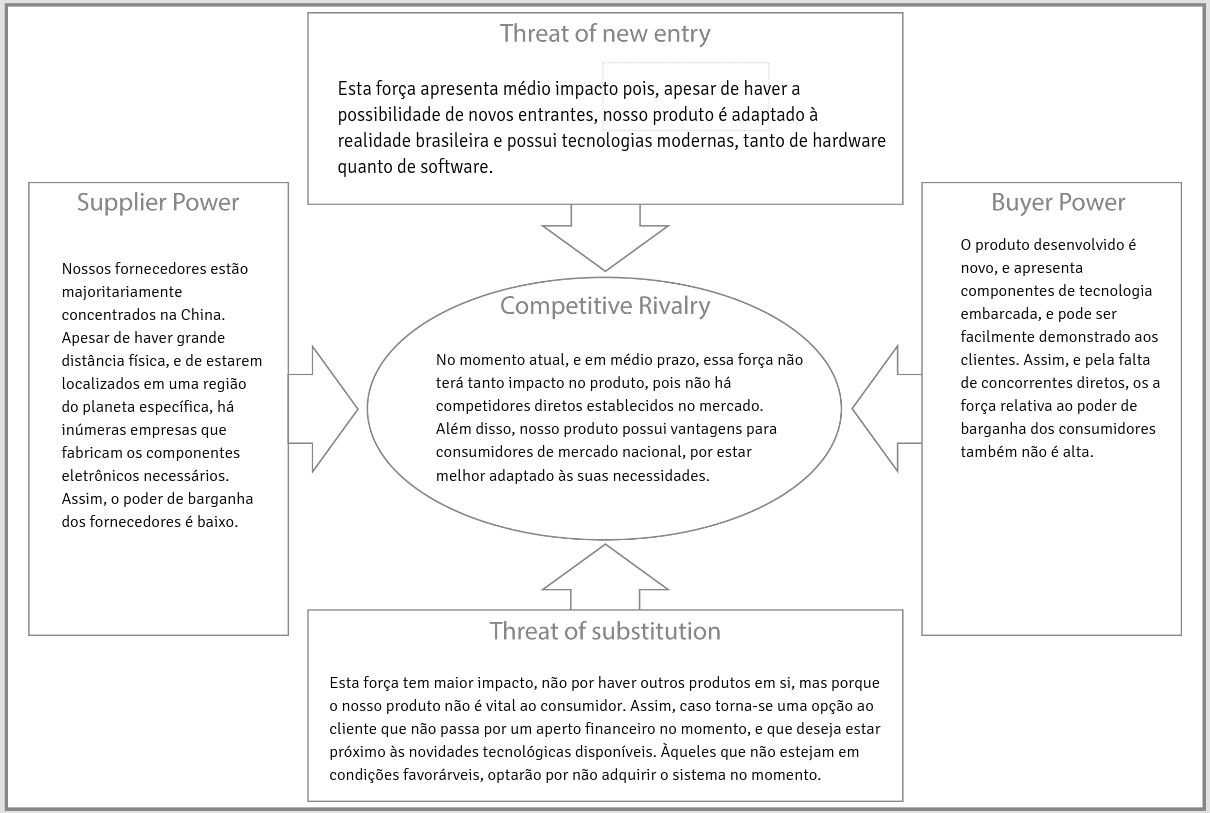
\includegraphics[width=0.8\textwidth]{porter}
	\end{center}
	\legend{Fonte: os autores}
\end{figure}

\subsection{Cadeia de Valor}

Conforme o definido por Michael Porter (Citar), para analisar todas as atividades desempenhadas pela empresa, com a finalidade de se criar vantagem competitiva em relação aos seus concorrentes, pode-se utilizar o modelo da Cadeia de Valor. Na \autoref{fig:cadeiaValor}, verifica-se a sua estrutura, que será detalhada em seguida.

\begin{figure}[H]
	\caption{\label{fig:cadeiaValor}Cadeia de Valor de Porter}
	\begin{center}
	    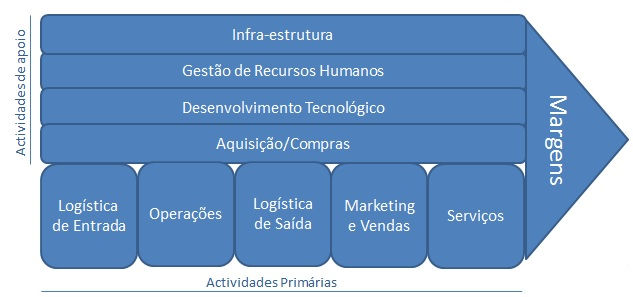
\includegraphics[scale=0.8]{cadeiaValor}
	\end{center}
	\legend{Fonte: CITAR http://www.gestaoporprocessos.com.br/o-modelo-de-cadeia-de-valor-de-michael-porter/}
\end{figure}

\begin{description}
    \item[Infraestrutura:]Todas as atividades necessárias para a empresa funcionar enquanto uma instituição. Emissões de relatórios, planejamentos, etc. fazem parte deste conjunto de atividades.

    \item[Gestão de Recursos Humanos:]Responsável pela manutenção dos servidores, e a contratação de novos profissionais, bem como resolução de possíveis conflitos internos.

    \item[Desenvolvimento Tecnológico:]Essencial na Hedwig, já que faz parte da base de nossos produtos, e é um fator determinante para que a empresa esteja sempre na liderança do mercado.

    \item[Aquisição/Compras:]Negociação com os fornecedores e todas as atividades relativas a obtenção de matéria-prima.

    \item[Logística de Entrada:]A matéria prima é importada da China, e é transportada de navio até a o porto de Santos, de onde seguirá para a empresa, por meio de uma empresa responsável pelo fretamento.

    \item[Operações:]Englobam as atividades de montagem física dos módulos, com a soldagem dos componentes nas placas de fenolite, e a instalação do microcontrolador.

    \item[Marketing e Vendas:]Atividades relacionadas com o oferecimento dos nossos produtos, tanto aos consumidores finais quanto lojas específicas.

    \item[Serviço:]Atividades de pós-venda e suporte, para que o consumidor esteja sempre satisfeito com os nossos produtos, e quaisquer problemas encontrados devem ser resolvidos prontamente.
\end{description}

\section{Aspectos Éticos e de Segurança}

% TODO

\section{Comércio Eletrônico}

Haverá comércio inicialmente através de parceiros estratégicos em contato direto (revendedores locais, como instaladores de sistemas de alarmes), e comércio eletrônico após obtenção de escala, em duas etapas distintas:
\begin{enumerate}
	\item Email: canal consolidado de pedidos e comunicação com fornecedores e clientes (reclamações e pós compra);
	\item \textit{Site}: portal próprio, protegido por https com certificado digital, para a gestão de relacionamento com clientes e fornecedores, buscando expansão do \textit{e-commerce} 
\end{enumerate}

\section{Social Business}

A publicidade será feita por página em redes sociais (Facebook), manutenção de página no GitHub, Canal no Youtube, Blog com tutoriais (e evolução do projeto). A ideia é fazer uma comunidade fiel ao conceito de casa conectada, através dos seguintes canais:
\begin{enumerate}
	\item \textbf{Facebook}: Usuários podem enviar feedbacks, requisições e espalhar anúncios de produtos prontos;
	\item \textbf{GitHub}: Usuários que gostam de programar podem interagir com o projeto (código livre);
	\item \textbf{Youtube}: Videos demonstrando funcionalidades e situações de uso, além de servir de suporte para o blog;
	\item \textbf{Blog}: Contém os vários tutoriais relativos aos diferentes usos dos módulos, além de notícias sobre a evolução do projeto (novas funcionalidades e módulos).
\end{enumerate}

\section{Inteligência de Negócios e Gestão de Riscos}

% TODO

Segue matriz SWOT para análise de riscos:

\begin{figure}[htb]
	\caption{\label{fig:SWOT}Matriz SWOT}
	\begin{center}
		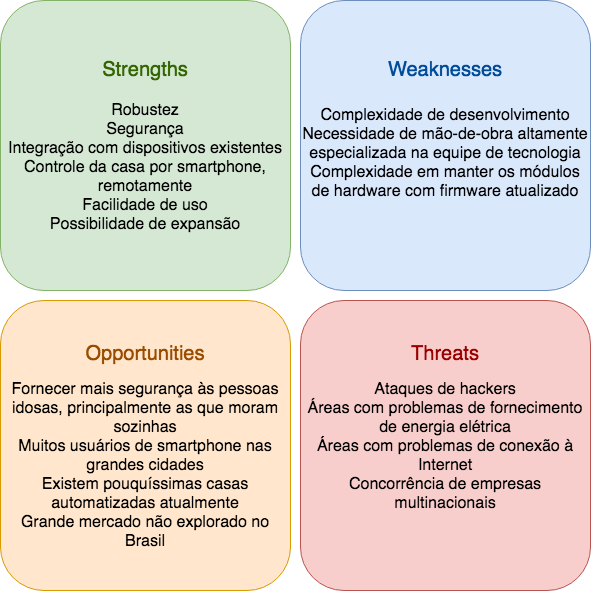
\includegraphics[scale=0.5]{SWOT}
	\end{center}
	\legend{Fonte: os autores}
\end{figure}